\chapter{Description and analysis of existing test framework} 
\label{Chapter3} 

Two emulators for the Serval mesh exist, one for testing the functionality of Serval DNA and Rhizome, and the other for testing LBARD. 
The first was built to test the functionality of the Serval mesh in its early days; when nodes were purely communicating over WiFi. 
This emulator is able to emulate multiple aspects of the Serval DNA software, from validating the database integrity to simulating WiFi communication between Serval nodes. 
Later, once LBARD was added to the Serval project, a second emulator was built that extended the code of the Serval DNA emulator.
This emulator performed similar functions to that of the Serval DNA emulator; testing internal LBARD functionality, and emulating radio communication between Serval nodes. 
While the LBARD emulator serves as an extension to the Serval DNA emulator - extending and overwriting functionality - there is currently no ability to run tests that feature both WiFi and radio links. 
\todo{change to more of an intro}


\section{Aims of test frameworks}
In a project like the Serval project, confidence in its performance is crucial - particularly if it will be used in disaster recovery efforts.
To achieve this, both the development team and potential users of the network need to be confident in its performance in a wide range of scenarios. 
While a significant portion of this will need to be done through field testing, this is simply unrealistic and vastly too expensive to perform to undergo on the level that the Serval network needs to be tested to.
To solve this, the Serval team have developed the Serval DNA and LBARD emulators, allowing them to effectively model the behavious of the Serval software in a wide range of scenarios without the prohibitive overhead cost and effort of field tests.

The two emulators have different goals: the Serval DNA emulator is purely for testing native Serval functionality - adding to Rhizome databases, WiFi synchronisation, and other core Serval functionality; while the LBARD emulator is designed for testing the functionality of LBARD and how it behaves when combined with Serval DNA.
\todo{Is this grammar right?}
The emulators are split in such a way for one simple reason; Serval DNA does not require LBARD to be running - or even installed - to function, however LBARD requires Serval DNA to be running to function.
Thus, it makes no sense to have an emulator for the Serval DNA emulator to be attempting to test LBARD code since they are discrete entities.
However, having the LBARD emulator extend from the Serval DNA emulator is done so that the emulators are running near-identical code, minimising the risk that the emulators are not working in similar ways.



\section{Serval DNA Test Framework}
The Serval DNA test framework is a bash script that serves as the basis of Serval testing.
It is able to test a wide range of functionality of the Serval software, from validating databases, to communicating with other Serval nodes over WiFi.

The framework serves as the basis for writing tests for the Serval network, with a large range of tests using this framework.
These tests are also bash scripts that import the necessary functions to run tests from the framework. 
The test framework provides functions for setting up and running tests, as well as handling features such as starting and stopping servald instances.
With this framework, these test scripts are able to model a wide range of Serval functionality, allowing for developers to easily and effectively write tests with a minimal amount of work needed.

The test framework is composed of three major parts; the test framework, the test definitions, and the test file.
The framework (\emph{testframework.sh}) provides the functions necessary to run tests, providing: command line argument parsing, running tests, stopping tests, monitoring log files, and more. 

The test definitions file (\emph{testdefs.sh}) provides specific functions that are needed for specific test files.
This file provides the functionality to setup, start, and stop serval instances, configure specific instances, and more.
When running specific types of tests, the \emph{testdefs.sh} file can be extended by other files such as in the case of the \emph{testdefs\_rhizome.sh} file. 
This allows for some functions provided in the testdefs file to be overwritten, allowing for different functionality depending on the type of test; this is of great use particularly when attempting to use different configurations than that provided by the original \emph{testdefs.sh} file

Finally, the test files themselves are where tests are defined. 
These files import the test definitions and test framework and define the environment and test conditions necessary to run tests. 

Running the tests is as simple as running the test file that tests the features you're looking for, the framework and definitions will be imported automatically.

\section{LBARD Test Framework}
The LBARD test framework extends the functionality of the Serval DNA test framework, however it overrides multiple functions to get it working with LBARD.
By overriding functions, the LBARD test framework is able to create Serval instances running with LBARD and is able to connect these instances through a fake radio interface called fakeradio.
Fakeradio monitors the LBARD radio outputs of each of the LBARD interfaces, and sends the packets it receives to the inputs of each of the LBARD radio input files, dependent on the rules defined when starting the fakeradio program.
The rules that can be sent to fakeradio allow test creators to define network layouts by denying all traffic between nodes unless specified otherwise, allowing for many radio topologies to be defined.
With the extended test framework, testers can develop tests for LBARD-based network topologies.
Fakeradio is able to simulate several radio interfaces including; RFD900, BarrettHF, and CodanHF.


When a test is run, the test framework starts the specified number of Serval instances, each with their own separate databases, configurations, and log files.
Then, LBARD instances are started for each of these instances, running simulated radio hardware (RFD900, BarrettHF, etc.) as defined in the test definition.
Finally, fakeradio is started and begins to listen to the output files of each of the LBARD interfaces, simulating the radio links between real devices, with configurable parameters such as packet loss.
Once a test is concluded, the framework collects all of the log files and outputs of the serval instances, LBARD instances, and fakeradio.
These are then collated into a single test log file, with every piece of data timestamped.
This way of running the tests has several benefits for the purpose of this Honours project; firstly, the test framework is running the real software that runs in a real-world scenario, with only the radio links being simulated; secondly, the framework collates all of this data into a single log file, greatly minimising the work that needs to be done in later stages of this project to extract events in a test from multiple log files.

\emph{Unless otherwise specified, when talking about the test framework in this document, we will be talking about the LBARD test framework.}


\subsection{Defining Tests}
Tests are defined in either the lbard (\emph{./lbard/tests/lbard}) or lbard\_size\_tests (\emph{./lbard/tests/lbard\_size\_tests}) file. 
These are both bash files that implement the LBARD test framework, and simply define what tests are to be run.
Tests are comprised of three basic components; a doc string with a brief description of what the test does, a 'setup' function that sets up the test environment, and finally, a 'test' function, that is run when the test is run.
The doc string is used when running tests and serves as feedback to the tester as to what test is currently being run.
The setup function is run before the test is conducted. This function serves to set up any necessary configurations for the running of this test. This is where the fakeradio rules are defined, files added to Serval instances, and any other necessary setup for a test.
Finally in the test function, the conditions for a successful test are defined. Once this function completes (or an error/fail/timeout is encountered), the test concludes.


This can be seen in Figure \ref{fig:testDefinition}. 
In this example, the setup function defines the fakeradio rules, then adds a single file of 50 bytes to the Serval instance A. 
In the test function, a function 'all\_bundles\_received' is defined, that simply checks if instance B received a bundle with the specified bundle ID and version. 
The test then waits until this bundle is received. 
If this bundle is received before the default timeout, the test will pass.

\begin{figure}
    \begin{centering}
        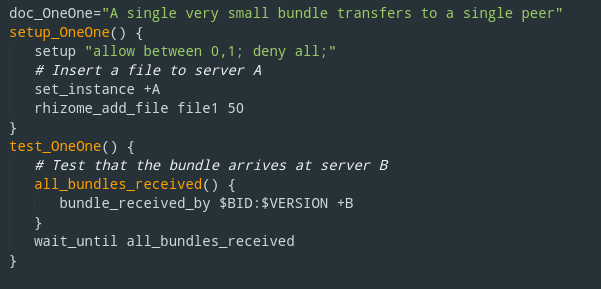
\includegraphics[width=14cm,height=20cm,keepaspectratio]{Figures/testdefinitionexample.png}
        \caption{Example of LBARD test definition}
        \label{fig:testDefinition}
    \end{centering}
\end{figure}

\subsection{Existing Tests}
Currently, 276 LBARD tests exist; 55 of these are in \emph{./tests/lbard} file, and 221 of these are in the \emph{./tests/lbard\_size\_tests} file.
While this may seem like a large number of tests, all of the tests in the \emph{lbard\_size\_tests} file follow the exact same structure - transferring a bundle from one node to three neighbours - with the only difference being the size of the bundle.
The bundle simply increases in size by 10 bytes for each tests from 6000 bytes to 8200 bytes.

In the main LBARD test file, there are only a handful of tests, with the majority of them being derivatives of different tests with mild changes. 
The majority of the tests in the LBARD test file are as follows, with slight difference in test variables:
\begin{itemize}
    \item Detect radio types (RFD900, BarrettHF, CodanHF)
    \item Setup for Outernet
    \item Outernet up-link tests with various sizes
    \item One peer to one peer with BarrettHF
    \item One peer to one peer with various sizes
    \item MeshMS with different packet loss
    \item File delivery with 3 hops over UHF (RFD900)
    \item 10 nodes sending, 10 receiving, various LBARD options
    \item 10 nodes sending, 10 receiving, various packet sizes
\end{itemize}




\section{Outputs}
Tests produce two main outputs; a PASS/FAIL status in the command line, and a log file.
This log file contains the outputs of all the programs run in the course of the test including Serval DNA and LBARD instances, fakeradio, and the test framework itself, with each line in the log file is timestamped.
The log files produced contain several pieces of infomation.
At the beginning of the file the name, result (pass/fail), and start/finish time of the test are listed.
Following that, the complete logs of each of the started subprocesses (LBARD, Serval DNA, etc.) are listed.

Tests can be configured to display more details log file infomation by setting specific flags in the configuration of the test.

\begin{figure}
    \begin{centering}
        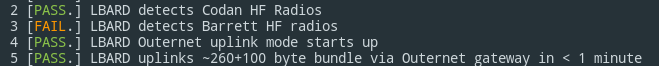
\includegraphics[width=14cm,height=20cm,keepaspectratio]{Figures/testOutput1.png}
        \caption{Example output of LBARD tests}
        \label{fig:exampleTest}
    \end{centering}
\end{figure}


As shown in \figurename{\ref{fig:exampleTest}} When a test is run, four possible status messages can be displayed; pass, fail, error, and fatal.

\emph{Pass} is simply when a test has fulfilled the requirements outlined in the test definition.

\emph{Fail} occurs when a test does not meet the requirements from a test definition but it is not due to an issue with the test or test definition. This may occur if a timeout elapses, or an output does not meet a success condition.

The \emph{error} status occurs when - during the process of running the test - an error occurs that stops the test from running correctly, such as LBARD failing to start properly, or being unable to start Serval DNA with the current configuration.

Finally, the \emph{fatal} status occurs files don't exist that should, commands are not available, or invalid options are passed to the test framework.



\section{Limitations}
While the emulators are able to test large portions of the Serval network, they have several limitations that drastically limit the usefulness of the emulators to effectively model real world situations.
The largest of these limitations is that it is currently not possible to model networks that use both WiFi as well as radio, limiting the testable scenarios to that of just WiFi, or just radio networks.
Further, as it is not possible for different radio methods to communicate with each other (i.e. you cannot connect a UHF radio and a HF radio ) without linking them with WiFi (as described in Chapter \todo{link to previous description of Serval network}) this further limits possible network topologies to networks of only a single radio type.
This is a huge limitation to modelling and testing Serval networks, as real Serval networks most likely will feature multiple communication types as best suit the needs of the network.
\todo{talk about Vanuatu example?; ref.} 
\todo{add ref.}

Another major limitation of the test frameworks is that there currently exists very few topologies that are being tested.
While the Serval DNA portion of the framework does feature various WiFi-exclusive topology tests including long node chains and a 6 node circular network these are relatively few and the only LBARD topology tests that exist are very minimal and basic.
Further, with the few topology tests that it does have, there is zero output in the log files that clearly state what the topology of the test is. 
Obviously, there are no currently existing topology tests that contain multiple radio types or WiFi/radio networks.

While the log files produced by the tests are extensive and contain a large amount of data that is helpful while debugging, it does have several drawbacks. 
Firstly, with just the log files and the Pass/Fail/Error output it is very difficult to work out what is going wrong - especially in initial stages of debugging network topologies.
Partially, this is due to the log files not being chronologically ordered, but instead ordered by what log file it is, and \emph{then} chronologically ordered.
This means that attempting to work out where an error occurred becomes a process of consistently switching places in the large log file.
When more detail has been located about the issue - such as which device it occurred on, then it is useful to go through the large log file.
Further, the log file has another draw back in that it becomes incredibly difficult to easily understand topology functionality or explain to others what an issue is to a lack of visual output.
This ties into the previously mentioned issue of difficulty determining where issues are occurring.

Finally, as topology tests have not been extensively tested, it is difficult to know how accurate these tests really are.
Without running tests in near-identical emulated and real scenarios it is very difficult to determine if the serval emulator is even properly modelling communication between devices. 
A lack of comparisons between real-world tests and emulated tests means that confidence in the results of emulated tests is minimal and presents a theoretical view of how the Serval mesh may work under given conditions. 


\section{How to improve}
To improve the LBARD test framework, multiple changes will need to be made.
The first of these is adding the ability to allows nodes to communicate over both WiFi and fakeradio. 
This step alone will drastically increase the scope of possible tests that can be conducted, as it will allow for tests of both WiFi and emulated fakeradio interface.
Further, this will allow for networks to utilise more than one type of radio communication.

With the ability to have multiple link types betwen Serval nodes, a much larger range of network topologies can be modelled and tested.
Adding more network topologies to the test framework will allow for a much more detailed testing, and will almost certainly uncover previously undiscovered issues with the Serval network as it has simply not been possible to test complicated network topologies before.

To improve on the ability to understand and communicate the functionality of specific Serval network topologies, some form of graphical output will need to be created, allowing for testers to see the network undergoing testing, as well as the packets and bundles moving around the network.
This will almost certainly prove beneficial to the Serval team on two fronts. 
Firstly, this will assist Serval developers in isolating and locating bugs in Serval networks by visually showing them the functioning of a network, supplementing the expansive log files that the frameworks produce.
Finally, this will almost certainly help with communicating issues between Serval team members, as it is considerably easier to explain network functionality with diagrams and visuals than by scrolling through log files.
\todo{This is kind of weak. Change this bit?}

Finally, once the emulator can model a variety of network topologies, the accuracy of the emulator should be determined.
To achieve this, the emulator should model a real-world Serval network and run various test on this network, and then those same tests should be run on a real-world implementation of this network.
This wil serve to validate the accuracy of the Serval emulator, as it is expected that modelling the same network should have near-identical results with minimal variance.